\documentclass[a4paper,11pt,twoside]{report}

% ==========================================================
% TITLE / AUTHOR -- fill these in yourself (see coordinator's
% MScThesisTemplate.tex for the pattern this follows).
% ==========================================================
\newcommand{\theTitle}{A Statistical Study of Mathematical Reasoning Errors in Large Language Models using Tree-of-Thought Reasoning}
\newcommand{\theShortTitle}{Mathematical Reasoning Errors in LLMs}
\newcommand{\theAuthor}{Anushree Mahesha}
\newcommand{\theShortAuthor}{A Mahesha}
% TODO: confirm your exact Department name, MSc programme title, and
% supervisor's name/title with your coordinator -- placeholders below.
\newcommand{\theDepartment}{Department of TODO}
\newcommand{\theProgramme}{MSc in TODO}
\newcommand{\theSupervisor}{Dr TODO}

% Bibliography style -- classic bibtex + abbrv, matching the coordinator's
% template exactly (simpler and faster to compile than biblatex+biber).
\usepackage{cite}
\bibliographystyle{abbrv}

% Page style
\usepackage[a4paper,top=2.5cm,bottom=2.5cm,outer=2.5cm,inner=2.5cm,includeheadfoot]{geometry}
\usepackage{fancyhdr}
\pagestyle{fancy}
\headheight=18pt
\footskip=24pt
\fancyhf{}
\renewcommand{\chaptermark}[1]{\markboth{}{#1}}
\fancyhead[RO,LE]{\bfseries \theShortTitle}
\fancyhead[LO,RE]{\bfseries \rightmark}
\fancyfoot[C]{\thepage}

% Spacing
\usepackage{setspace}
\usepackage{parskip}

% Maths typesetting
\usepackage{amsmath}
\usepackage{amsfonts}
\usepackage{amssymb}
\usepackage{booktabs}

% Graphics -- figures can go in ./Figures/, or point directly at the
% project's generated outputs so regenerated figures don't need copying.
\usepackage{graphicx}
\graphicspath{{./}{./Figures/}{../outputs/figures/}}

% TikZ/pgfplots, as in the coordinator's template
\usepackage{tikz}
\usepackage{pgfplots}
\pgfplotsset{compat=1.15}
\usetikzlibrary{calc}
\usetikzlibrary{plotmarks}
\usetikzlibrary{patterns}
\usetikzlibrary{shapes}
\usetikzlibrary{positioning}

\usepackage[english]{babel}
\usepackage{hhline}

% User-defined commands, as in the coordinator's template
\newcommand{\dee}{\mathrm{d}}
\newcommand{\Dee}{\mathrm{D}}
\newcommand{\diff}[2]{\frac{\mathrm{d} #1}{\mathrm{d} #2}}
\newcommand{\ddiff}[2]{\frac{\mathrm{d}^2 #1}{\mathrm{d} #2^2}}
\newcommand{\pdiff}[2]{\frac{\partial #1}{\partial #2}}
\newcommand{\pddiff}[2]{\frac{\partial^2 #1}{\partial #2^2}}
\newcommand{\mdiff}[2]{\frac{\mathrm{D} #1}{\mathrm{D} #2}}
\newcommand{\ie}{\emph{i.e.}\ }
\newcommand{\eg}{\emph{e.g.}\ }
\newcommand{\etc}{\emph{etc.}}
\newcommand{\etal}{\emph{et al.}\ }
\newcommand{\etalp}{\emph{et al.}}
\newcommand{\floor}[1]{\left\lfloor #1 \right\rfloor}
\newcommand{\ceil}[1]{\left\lceil #1 \right\rceil}

\usepackage{hyperref}
\hypersetup{
    unicode=true,
    pdftoolbar=true,
    pdfmenubar=true,
    pdffitwindow=true,
    pdftitle={\theTitle},
    pdfauthor={\theShortAuthor},
    pdfnewwindow=true,
    colorlinks=true,
    linkcolor=red,
    citecolor=red,
    filecolor=blue,
    urlcolor=blue,
}

\title{\theTitle}
\author{\theAuthor}
\date{\today}

\begin{document}

\singlespacing

\hypersetup{pageanchor=false}
\begin{titlepage}
    \quad
    \vspace{1.25cm}
    \begin{center}
        
\includegraphics[scale=0.2]{UL_logo.png}
    \end{center}

    \begin{center}
        \vspace{1.5cm}
        \begin{minipage}{0.8\textwidth}
            \begin{center}
                \LARGE \bfseries \theTitle \\
            \end{center}
        \end{minipage}

        \vspace{2.5cm}
        \vspace{3.5cm}

        \begin{minipage}{0.8\textwidth}
            \begin{center}
                \Large \theAuthor \\
                \large \theDepartment \\
                University of Limerick \\
                \vspace{0.5cm}
                \large Supervisor \\
                \theSupervisor
            \end{center}
        \end{minipage}

        \vspace{2.5cm}

        \begin{minipage}{0.8\textwidth}
            \begin{center}
                \large MSc Thesis \\
                \textit{\theProgramme} \\
                \today
            \end{center}
        \end{minipage}

        \vfill
    \end{center}
\end{titlepage}

% Single spacing, matching the explicit "45-75 pages, based on using 11pt
% font and single line spacing" instruction -- the official template file
% uses 1.5 spacing instead; flagged as a genuine inconsistency between the
% two official documents, single spacing chosen since it's the more
% specific, directly-stated rule. Switch to \onehalfspacing here if your
% coordinator says otherwise.
\singlespacing
\hypersetup{pageanchor=true}
\setcounter{page}{1}
\pagenumbering{roman}

% ---------- Declaration ----------
\fancyhead[LO,RE]{\bfseries Declaration}
\chapter*{Declaration}
\addcontentsline{toc}{chapter}{Declaration}
I hereby declare that this dissertation is entirely my own work and has not
been submitted, in whole or in part, for any other academic award at this
or any other institution. Where the work of others has been used or
referenced, it has been fully acknowledged.

\vspace{2cm}
\noindent Signed: \underline{\hspace{6cm}} \quad Date: \underline{\hspace{4cm}}

\newpage

% ---------- Acknowledgements ----------
\fancyhead[LO,RE]{\bfseries Acknowledgements}
\chapter*{Acknowledgements}
\addcontentsline{toc}{chapter}{Acknowledgements}
% TODO: write yourself.

\newpage

% ---------- Abstract (≤200 words per the MSc outline) ----------
\fancyhead[LO,RE]{\bfseries Abstract}
\chapter*{Abstract}
\addcontentsline{toc}{chapter}{Abstract}
% TODO: write yourself, last, once Results/Discussion are final. Max 200 words.

\vspace{30pt}
\emph{\textbf{Keywords:} Large Language Models, Mathematical Reasoning, Chain-of-Thought, Tree-of-Thought, Error Analysis}

\newpage

\parskip=12pt

\fancyhead[LO,RE]{\bfseries Contents}
\addcontentsline{toc}{chapter}{Table of contents}
\tableofcontents

\newpage
\fancyhead[LO,RE]{\bfseries List of figures}
\addcontentsline{toc}{chapter}{List of figures}
\listoffigures

\newpage
\fancyhead[LO,RE]{\bfseries List of tables}
\addcontentsline{toc}{chapter}{List of tables}
\listoftables

\newpage
\fancyhead[LO,RE]{\bfseries List of Abbreviations}
\chapter*{List of Abbreviations}
\addcontentsline{toc}{chapter}{List of Abbreviations}
\begin{tabular}{ll}
    AIME & American Invitational Mathematics Examination \\
    CoT  & Chain-of-Thought \\
    LLM  & Large Language Model \\
    RQ   & Research Question \\
    ToT  & Tree-of-Thought \\
\end{tabular}

\newpage
\fancyhead{}
\renewcommand{\chaptermark}[1]{\markboth{#1}{}}
\fancyhead[LO,RE]{\bfseries \leftmark}
\fancyhead[RO,LE]{\bfseries \theShortTitle}

\pagenumbering{arabic}

% ==========================================================
% CHAPTERS -- per the MSc outline: Introduction, Literature Review,
% Statistical/Mathematical Methodology, Application/Case Study, Results,
% Discussion and Conclusion (merged into one chapter per the outline's
% "as appropriate" flexibility, given the 45-75 page target).
% ==========================================================
\chapter{Introduction}
\label{chap:introduction}

% YOU WRITE THIS CHAPTER. Notes below are structure/content pointers only,
% not sentences to copy. Ask me to explain any of these before you write
% about them.

\section{Overview}

Large Language Models (LLMs) have become increasingly capable of solving
complex reasoning tasks, including mathematical problem solving, making
them valuable for applications such as intelligent tutoring systems,
educational technologies, and decision-support tools. As these models are
increasingly used in domains that require reliable multi-step reasoning,
understanding not only their final performance but also the reasoning
process leading to their answers has become an important area of research.

This dissertation investigates the mathematical reasoning performance of
three Large Language Models---Gemini Flash Lite, GPT-OSS-120B, and Mistral
Large---using two reasoning-based prompting strategies: Chain-of-Thought
(CoT) and Tree-of-Thought (ToT). The study evaluates model performance on a
curated dataset of mathematical problems drawn from the Hendrycks MATH
dataset and selected American Invitational Mathematics Examination (AIME)
questions. Beyond measuring answer correctness, the research analyses the
types of mathematical reasoning errors produced by each model, identifies
where within the reasoning process these errors occur, and compares the
effectiveness and computational cost of the two prompting strategies.

This chapter introduces the research by presenting the motivation for the
study, defining the research problem, outlining the research questions and
objectives, and summarising the main contributions of the dissertation. It
concludes with an overview of the remaining chapters, providing the
context for the methodology, experimental evaluation, statistical
analysis, and discussion presented throughout the dissertation.

\section{Motivation}

Large Language Models (LLMs) have become increasingly capable of solving
complex reasoning tasks and are now widely used in applications such as
intelligent tutoring systems, educational technologies, and
decision-support tools. As these models continue to be integrated into
domains that require reliable mathematical reasoning, understanding the
quality of their reasoning process has become increasingly important.
Mathematical problem solving differs from many other natural language
tasks because it requires logically consistent multi-step reasoning, where
an error in an intermediate step can invalidate the entire solution.
Consequently, evaluating the reasoning capabilities of LLMs is essential
for assessing their reliability and suitability for real-world
applications.

The growing use of reasoning-based prompting techniques has created new
opportunities to improve the mathematical performance of LLMs.
Chain-of-Thought (CoT) prompting encourages models to generate intermediate
reasoning steps, while Tree-of-Thought (ToT) prompting extends this process
by exploring multiple reasoning paths before selecting a final solution. As
these prompting strategies become increasingly popular, it is important to
understand not only whether they improve answer accuracy but also how they
influence reasoning behaviour, execution time, and mathematical
problem-solving performance. This motivates the need for a systematic
evaluation of different Large Language Models across diverse mathematical
problems using structured prompting strategies.

\section{Problem Statement}

Large Language Models (LLMs) have demonstrated strong performance on
mathematical reasoning benchmarks, with most existing studies evaluating
their capabilities using overall answer accuracy. Although accuracy is an
important performance indicator, it provides only a high-level measure of
model performance and offers limited insight into the reasoning process
that leads to a solution. As a result, existing evaluations often fail to
explain the nature of reasoning failures, the stage at which errors occur,
or how different prompting strategies influence mathematical reasoning
behaviour.

Furthermore, while reasoning-based prompting techniques such as
Chain-of-Thought (CoT) and Tree-of-Thought (ToT) have been widely adopted
to improve mathematical reasoning, many studies compare these approaches
using descriptive accuracy metrics alone. Such comparisons provide limited
evidence regarding whether observed differences in performance are
statistically meaningful. In addition, there is relatively little work
that simultaneously analyses reasoning error types, identifies where
errors occur within the reasoning process, and evaluates the effectiveness
of prompting strategies across multiple Large Language Models using a
controlled experimental design.

To address these limitations, this dissertation presents a systematic
study of mathematical reasoning in Large Language Models using a curated
dataset of mathematical problems covering multiple domains and difficulty
levels. Three Large Language Models are evaluated using both
Chain-of-Thought and Tree-of-Thought prompting strategies. In addition to
measuring answer correctness, the study analyses reasoning error types,
error locations, execution time, and model performance, followed by
appropriate statistical analyses to compare the behaviour of different
models and prompting strategies. By moving beyond aggregate accuracy, this
research aims to provide a more comprehensive understanding of the
reasoning capabilities and limitations of contemporary Large Language
Models.

\section{Research Questions}

This dissertation investigates the mathematical reasoning capabilities of
Large Language Models by addressing the following research questions.

\textbf{RQ1:} What are the most common types of mathematical reasoning
errors made by Large Language Models, and does the distribution of error
types differ across models?

This research question examines whether different Large Language Models
exhibit distinct patterns of mathematical reasoning errors. Since both the
evaluated model and the error type are categorical variables, the study
employs the Chi-square test of independence to determine whether the
observed distribution of error categories differs significantly across
models. Where expected cell frequencies are small, the results are
interpreted with caution because the Chi-square approximation becomes less
reliable. The assumptions and limitations of the Chi-square test,
including the presence of small expected cell counts in this study, are
discussed further in the Methodology chapter.

\textbf{RQ2:} At what stage of the reasoning process do mathematical
reasoning errors first occur, and does this differ across models or
prompting strategies?

This research question investigates whether different models or prompting
strategies tend to fail earlier or later during the reasoning process. The
analysis compares the relative position of the first reasoning error
within generated solutions. As the error-position measurements are not
assumed to follow a normal distribution, the Kruskal--Wallis test is
employed to compare error locations across multiple independent groups.

\textbf{RQ3:} Does Tree-of-Thought prompting significantly improve
mathematical reasoning performance compared with Chain-of-Thought
prompting for each Large Language Model?

This research question evaluates whether Tree-of-Thought (ToT) prompting
produces significantly different answer correctness compared with
Chain-of-Thought (CoT) prompting. Since every mathematical problem is
solved using both prompting strategies for the same model, the
observations are paired rather than independent. Therefore, McNemar's
Exact Test is employed to compare the two prompting strategies while
accounting for the paired experimental design.

Together, these research questions investigate complementary aspects of
mathematical reasoning in Large Language Models. RQ1 analyses the types of
reasoning errors produced by different models, RQ2 examines where
reasoning failures occur within the solution process, and RQ3 evaluates
the effectiveness of two reasoning-based prompting strategies.
Collectively, these questions provide a comprehensive assessment of
mathematical reasoning that extends beyond conventional accuracy-based
evaluations.

\section{Thesis Outline}

The remainder of this dissertation is organised as follows.

\textbf{Chapter 2 -- Literature Review} reviews the existing literature on
Large Language Models (LLMs) and mathematical reasoning. It discusses
Chain-of-Thought (CoT) and Tree-of-Thought (ToT) prompting strategies,
benchmark datasets including Hendrycks MATH and the American Invitational
Mathematics Examination (AIME), and recent approaches to automated
evaluation using LLM-as-a-Judge methodologies.

\textbf{Chapter 3 -- Statistical Methodology} presents the research
methodology adopted in this study. It describes the dataset construction
process, model selection, Tree-of-Thought implementation, answer
evaluation pipeline, error classification framework, and the statistical
methods used to address each of the research questions.

\textbf{Chapter 4 -- Application and Case Study} describes the
implementation of the experimental pipeline used to evaluate the
finalised dataset. It provides a detailed walkthrough of the evaluation
dataset, explains the collection of 786 model responses across different
models and prompting strategies, and describes the data quality assurance
procedures applied to ensure the reliability and consistency of the
experimental results.

\textbf{Chapter 5 -- Results} presents the experimental findings and
statistical analyses. The chapter reports the results for each research
question, compares model performance under Chain-of-Thought and
Tree-of-Thought prompting, and presents analyses of execution time,
answer correctness, reasoning errors, and other evaluation metrics.

\textbf{Chapter 6 -- Discussion and Conclusion} interprets the
experimental findings in relation to the research questions and existing
literature. It discusses the limitations of the study, highlights its key
contributions, provides recommendations for future research, and
concludes the dissertation by summarising the overall findings and their
implications.

\chapter{Literature Review}
\label{chap:literature}

% YOU WRITE THIS CHAPTER. Ask me to explain any paper/concept below before
% you write about it -- I can summarise a paper's actual contribution for
% you to then describe in your own words, but I won't write the review text.

\section{Prompting Strategies for Reasoning}
\subsection{Chain-of-Thought Prompting}
% \cite{wei2022chain} -- ask me what this paper actually showed and why
% it matters as your baseline condition.

\subsection{Tree-of-Thought Prompting}
% \cite{yao2023tree} -- ask me to explain the full tree-search design vs.
% the reduced-scale multi-branch version actually implemented here, and
% why that's a defensible scope decision to state explicitly, not hide.

\section{Mathematical Reasoning Benchmarks}
\subsection{The MATH Dataset}
% \cite{hendrycks2021measuring}

\subsection{AIME as a Benchmark Source}
% \cite{maa_aime} -- also: why AIME for the Hard tier specifically, and
% the data-contamination risk of any public competition-math benchmark.

\section{LLM-as-Judge Evaluation}
% \cite{zheng2023judging} -- and the self-evaluation bias risk this
% specific project has (Gemini judges Gemini's own responses), and how
% the neutral-judge validation sample addresses it.

\section{Error Analysis of LLM Mathematical Reasoning}
% Needs an actual literature search -- ask me to help you find and
% summarise papers that classify or localise LLM reasoning errors
% specifically (not just accuracy benchmarks), so you can position this
% thesis's contribution against them.

\section{Summary}
% Tie the sections above together into "here's the gap, here's what
% this thesis does about it."

\chapter{Methodology}
\label{chap:methodology}

This chapter explains the methods used in this study. It describes how
the evaluation dataset was built, which Large Language Models were chosen
and why, how the Chain-of-Thought and Tree-of-Thought prompting
strategies were designed, how answer correctness was judged, which
statistical tests were used for each research question, how the
error-judging process was set up, and the limitations of these methods.

\section{Dataset Construction}
\label{sec:dataset}

The evaluation dataset includes 131 mathematical problems, grouped into
three difficulty levels (Easy, Medium, Hard) and four categories: Algebra,
Number Theory, Probability, and Combinatorics. Table~\ref{tab:composition}
lists the exact breakdown.

\begin{table}[H]
  \centering
  \caption{Dataset composition by category and difficulty level.}
  \label{tab:composition}
  \begin{tabular}{lrrrr}
    \toprule
    Category & Easy & Medium & Hard (AIME) & Total \\
    \midrule
    Algebra          & 10 & 10 & 16 & 36 \\
    Number Theory    & 10 & 10 & 11 & 31 \\
    Probability      & 10 & 10 & 8  & 28 \\
    Combinatorics    & 10 & 10 & 16 & 36 \\
    \midrule
    \textbf{Total}   & \textbf{40} & \textbf{40} & \textbf{51} & \textbf{131} \\
    \bottomrule
  \end{tabular}
\end{table}

\begin{figure}[H]
  \centering
  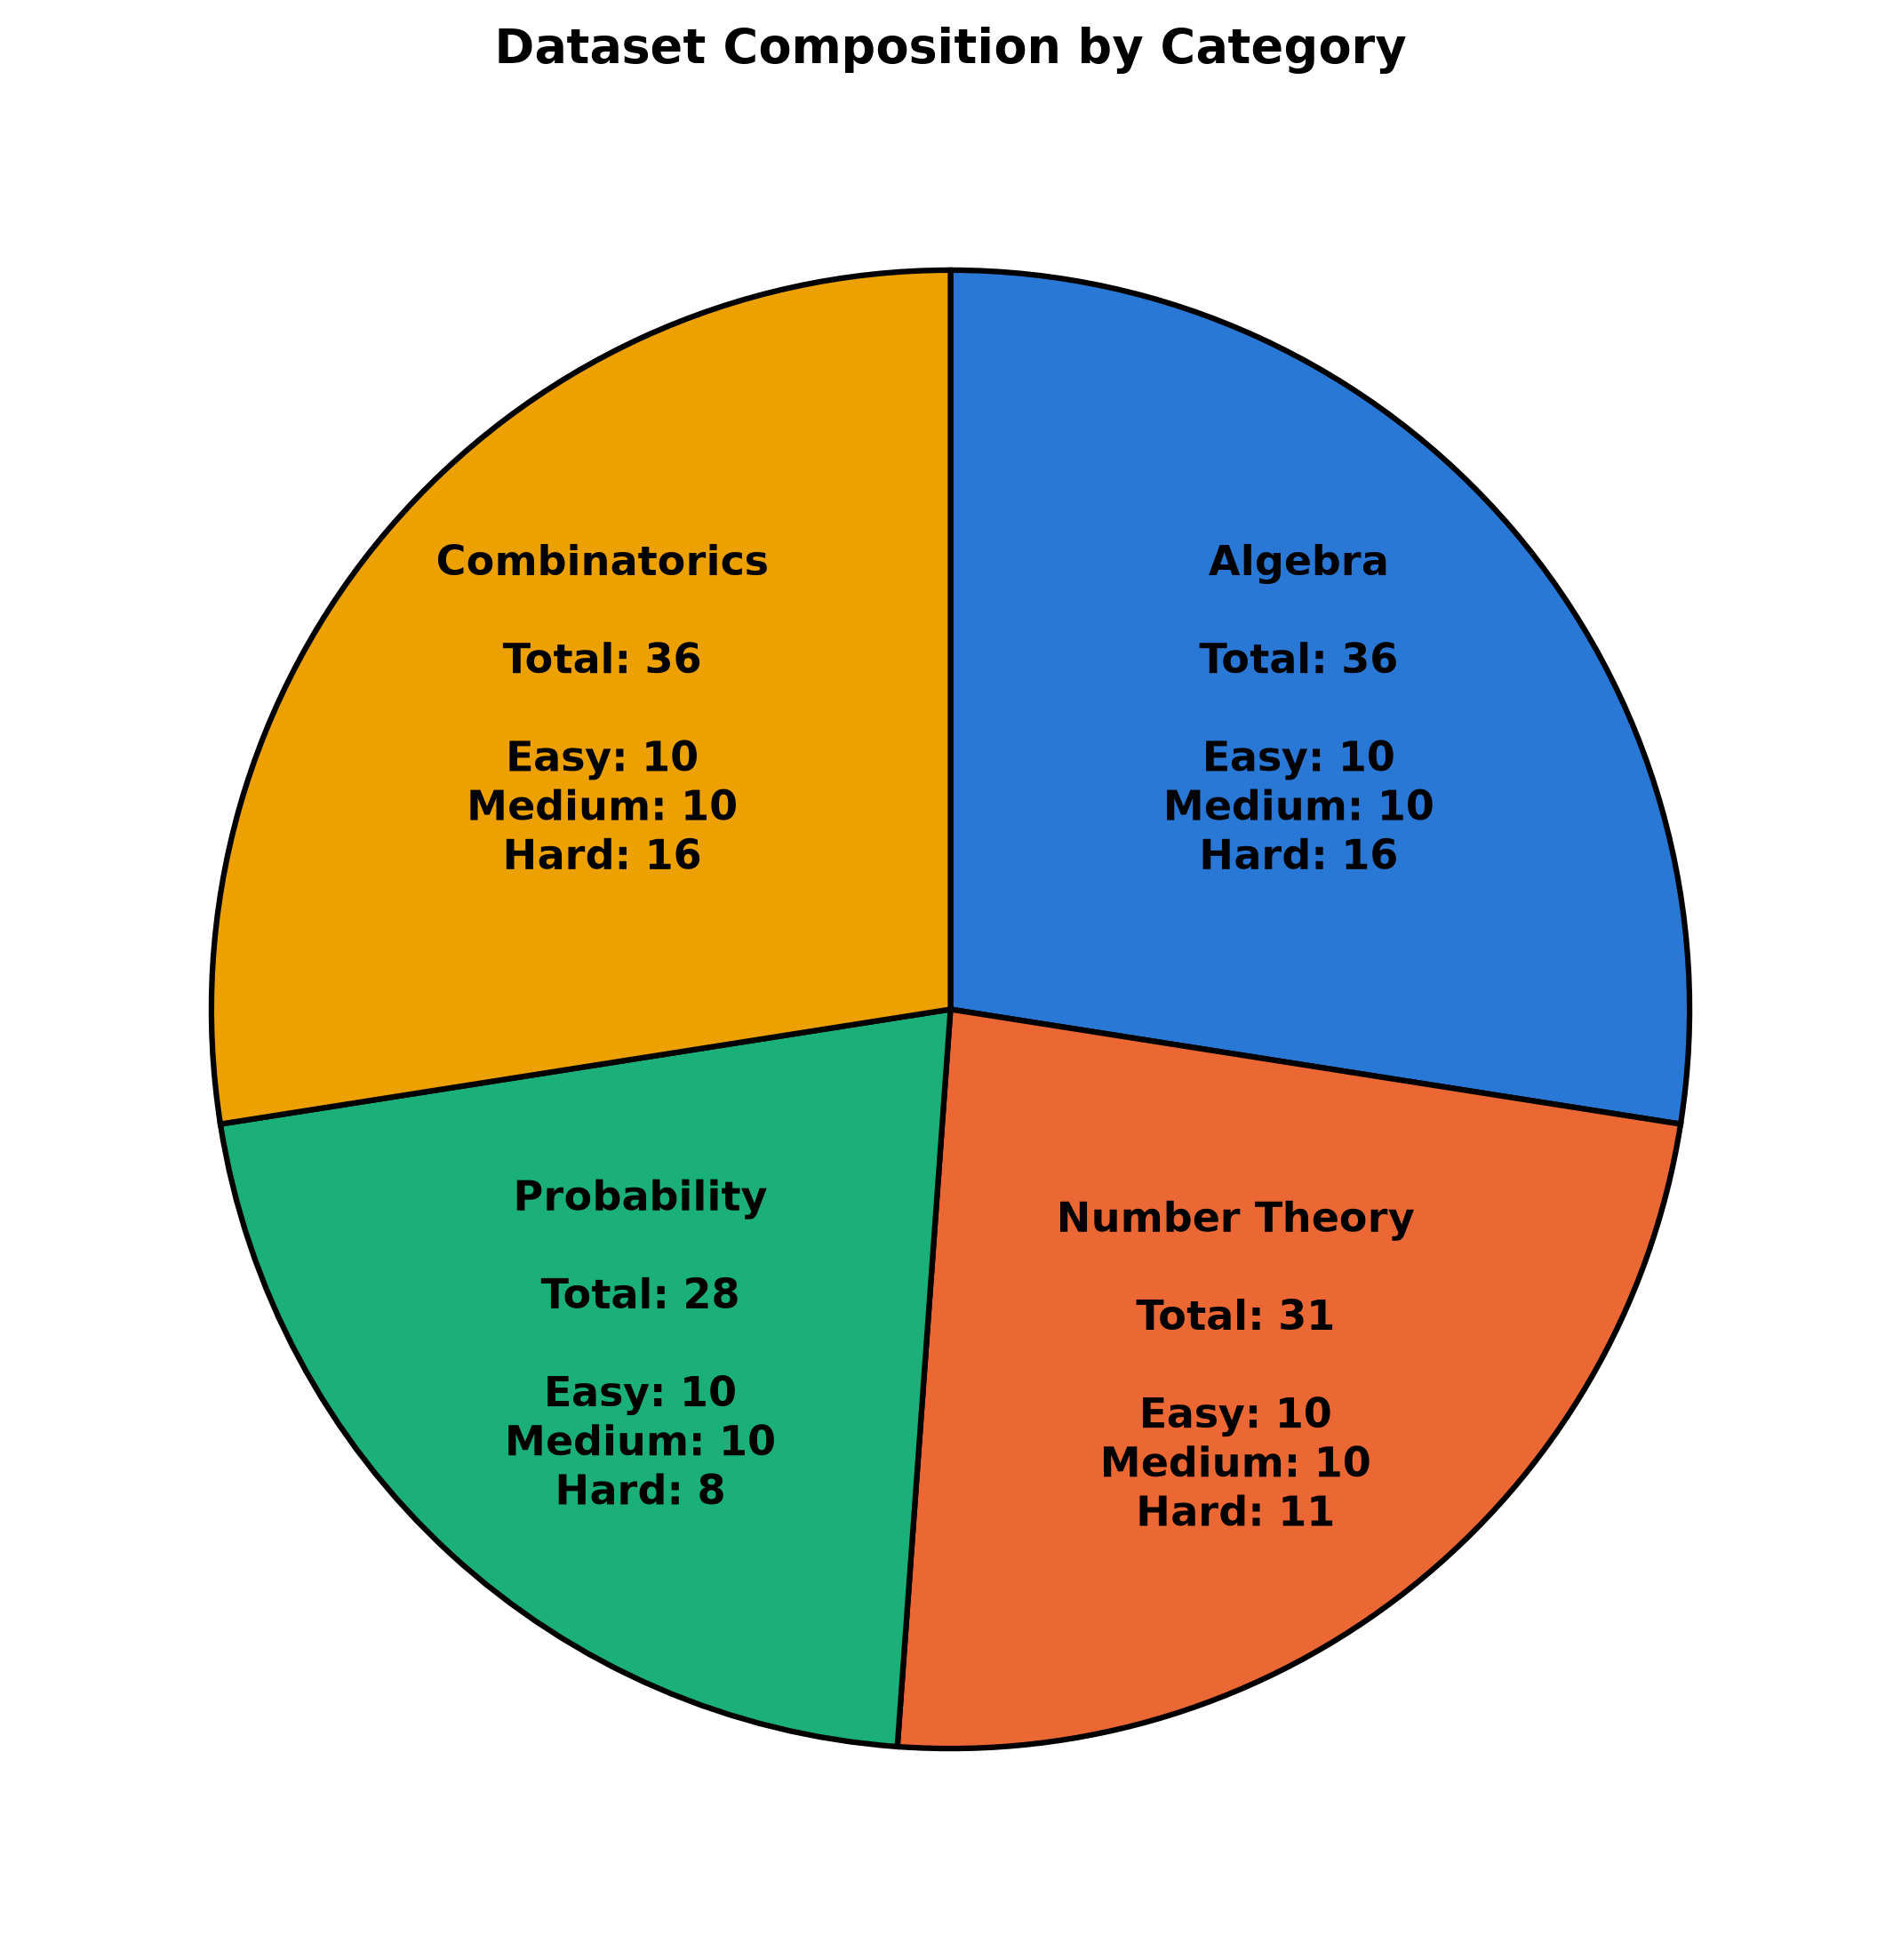
\includegraphics[width=0.7\textwidth]{dataset_composition_pie.png}
  \caption{Dataset composition by difficulty tier and category.}
  \label{fig:dataset-composition-pie-methodology}
\end{figure}

The Easy and Medium levels come from Hendrycks MATH, with exactly 10
questions per category in each level (using seed 25116096). These match
Hendrycks Levels 1--2 for Easy and Levels 3--4 for Medium. The Hard level
uses only questions from AIME.

The Hard level uses AIME questions only, rather than also including
Hendrycks MATH Level 5. AIME is a single, consistent competition-mathematics
source with a uniform integer answer format (0--999), which keeps
answer-parsing and grading consistent across the whole Hard tier. Hendrycks
MATH Level 5 is a separate item bank with a different answer format
(including fractional answers) and no independent validation that its
internal ``Level 5'' label represents the same difficulty as an AIME
problem. Mixing the two sources under one difficulty label would risk
treating non-comparable item banks as equivalent, so the Hard level was
restricted to AIME only.

The 51 Hard-level questions were drawn from six AIME contests: 2024 I,
2024 II, 2025 I, 2025 II, 2026 I, and 2026 II. The number of questions in
each Hard-level category is intentionally uneven, reflecting how many
questions of each category were available and labelled across these six
contests. Probability is limited to 8 questions because that is all the
AIME Probability questions available and labelled for this project. The
other three categories were not reduced to match. Reducing them would
have meant losing useful data without any real benefit, so the imbalance
is handled as a covariate in the analysis instead of forcing equal
numbers.

For most analyses in this study, the Hard tier is further restricted to
a fixed, seeded random sample of 40 of its 51 questions (seed 25116096),
matching the fixed size of the Easy and Medium tiers (40 questions each).
This gives a consistent, equal-sized pool of 40 questions per difficulty
tier -- 120 questions in total, so that no single tier's larger
question count disproportionately influences comparisons across tiers.
This balanced 120-question pool is used throughout this dissertation's
analyses unless otherwise stated. The one deliberate exception is the
per-question correctness matrix (Section~\ref{sec:question-correctness}),
which uses the full 51 Hard-tier questions (131 questions in total) to
show every curated question rather than a sample of them.

\section{Models}
\label{sec:models}

This study evaluates three large language models: Gemini Flash Lite
(\texttt{gemini-flash-lite-latest}, resolving to
\texttt{gemini-3.5-flash-lite}), GPT-OSS-120B (\texttt{openai/gpt-oss-120b},
via Groq), and Mistral Large (\texttt{mistral-large-latest}, resolving to
Mistral Large 3, \texttt{mistral-large-2512}). Each model is accessed via
its provider's free-tier API.

Gemini was included to ensure diversity among model providers. Groq hosts
open-weight models, originally from Meta's Llama family and later
OpenAI's GPT-OSS, while Mistral AI offers its proprietary Mistral-family
models. Including Gemini introduces a model from Google's family,
avoiding reliance on adjacent open-weight or single-vendor lineages. The
specific Groq and Mistral models were chosen after an earlier review
determined that the initially planned Llama-3.3-70B (Groq) and Mistral
Small performed inadequately on AIME-level problems. Additionally,
Llama-4-Maverick/Scout, the intended replacement on Groq, was deprecated.
GPT-OSS-120B was selected as Groq's recommended migration target for
these deprecated models.

All models are run with temperature set to 0, ensuring deterministic
responses for identical prompts. Two of the three models, Gemini and
GPT-OSS-120B, provide an internal control for ``thinking effort'' or
``reasoning effort.'' Both are set to their lowest available settings
(Gemini: \texttt{thinking\_level = "minimal"}; GPT-OSS-120B:
\texttt{reasoning\_effort = "low"}) and remain constant across both
Chain-of-Thought and Tree-of-Thought conditions. This control is
particularly relevant for RQ3. If this setting were allowed to vary,
differences in accuracy between Chain-of-Thought and Tree-of-Thought
could result from changes in internal reasoning budget rather than the
prompting strategy. Fixing the setting at its minimum value controls for
this confound, though it does not eliminate it entirely. This approach
does not guarantee the absence of internal reasoning, but ensures that
any such reasoning remains consistent across conditions. Mistral Large
does not expose an equivalent control and is used as a standard instruct
model throughout.

\section{Prompting Strategies}
\label{sec:prompting}
\subsection{Chain-of-Thought}

In the Chain-of-Thought setup, the model answers each question in a
single call. The model receives the problem and is instructed to explain
its reasoning step by step, concluding with a final answer in a
specified format.

This approach follows the standard single-pass Chain-of-Thought design,
in which one call produces a complete reasoning process and a final
answer. All outputs are generated at temperature 0 to guarantee
consistency. The prompt template standardises the output format,
enabling uniform parsing of responses among different models:

\begin{quote}
\ttfamily\small
Solve the following mathematics problem.\\
\\
Show your reasoning as clear, numbered steps.\\
\\
Format your response exactly as:\\
\\
Step 1: ...\\
Step 2: ...\\
Step 3: ...\\
\\
Final Answer: <answer>\\
\\
Problem:\\
\{question\}
\end{quote}

\subsection{Tree-of-Thought Design}
\label{sec:tot-design}

In the Tree-of-Thought setup, the model generates three independent
candidate solutions, referred to as branches. Subsequently, an
additional call selects the optimal branch. Thus, four calls are
executed per question, compared with the single call used in
Chain-of-Thought (CoT) prompting.

For each of the three branches, the model uses the same step-by-step
prompt as in CoT, with an additional instruction: each response is
explicitly labelled as a separate solution attempt (e.g., ``this is one
independent solution attempt, attempt N of 3''). The model is instructed
to commit to a single approach for each attempt, avoiding hedging
between methods. Branches are generated at a temperature of 0.7, rather
than 0, to promote diversity among solutions. A temperature of 0 would
result in nearly identical outputs, reducing the effectiveness of
comparative evaluation. Employing a moderate temperature ensures that
the branches represent genuinely distinct solutions.

After generating all three branches, the model performs an additional
call at temperature 0 to maintain consistency. During this step, the
model reviews the complete text of all three candidate solutions and
evaluates which branch demonstrates the most mathematically sound
reasoning. The model is instructed to select the branch with the
strongest justification, rather than defaulting to the most frequently
occurring answer in cases of disagreement among branches:

\begin{quote}
\ttfamily\small
Evaluate each candidate branch for mathematical soundness. Select the
ONE branch most likely to be correct and well-reasoned. If multiple
branches reach the same final answer through valid reasoning, prefer
the clearest derivation. If branches disagree, select based on which
reasoning is most rigorous and free of errors --- do not simply pick
the majority answer without checking the reasoning.
\end{quote}

It returns the number of the chosen branch and a brief explanation
(``Selected Branch: \texttt{<branch number>}'', ``Justification:
\texttt{<one sentence, maximum 25 words>}''). The full text of the
selected branch is then used just like a CoT response. If this selection
response cannot be parsed into a branch number, for example if the model
does not follow the requested output format, the pipeline falls back to
using the first generated branch rather than failing the
run.\footnote{Implemented in \texttt{src/parser/response\_parser.py}.}
This is a deliberate robustness choice: a single malformed selection
call degrades gracefully to a specific, predictable branch rather than
discarding the entire question's data or crashing the pipeline mid-run.

As mentioned in Chapter~\ref{chap:literature}, this version of
Tree-of-Thought is simpler than the full design by Yao et
al.~\cite{yao2023tree}. It does
just one round of branching and one selection step, instead of searching
and pruning at every reasoning stage. This approach keeps the number of
calls per question fixed at four, making costs predictable, but it means
the model does not explore or backtrack within a branch after it is
created.

\section{Answer Evaluation}
\label{sec:answer-eval}

Answer correctness is determined by an automated evaluator rather than
manual grading, since the study involves 786 model responses. Before
comparison, both the ground-truth answer and the model's extracted final
answer are passed through a normalisation step that strips formatting
artefacts that would otherwise cause two mathematically identical answers
to be marked as different: code fences and bold markers, commas, dollar
signs, LaTeX inline-math delimiters, \texttt{\textbackslash text\{\}} and
\texttt{\textbackslash boxed\{\}} wrappers, and LaTeX fraction notation
(\texttt{\textbackslash frac\{a\}\{b\}}, including the brace-less
shorthand \texttt{\textbackslash frac12}) converted to plain division
(\texttt{a/b}). A literal percent sign is converted to its decimal
equivalent (e.g. ``10\%'' to $0.1$) only when the answer is purely a
number followed by \%, so that a percent sign appearing elsewhere in an
answer is not misinterpreted. Mixed numbers such as ``2 1/3'' are detected
and converted to their decimal value before general normalisation runs,
since normalisation removes whitespace and would otherwise collapse
``2 1/3'' into the digit string ``21/3''.

After normalisation, two answers are compared using three methods, and
are considered correct if any one of them agrees:

\begin{enumerate}
  \item \textbf{Numeric comparison}: both answers are converted to
  floating-point numbers (handling plain integers, decimals, and
  fractions) and compared with a small numerical tolerance, so that
  trivial floating-point representation differences are not counted as
  errors.
  \item \textbf{Symbolic comparison}: both answers are parsed as
  algebraic expressions using SymPy, and are considered equal if their
  difference simplifies to zero. This allows answers that are
  algebraically equivalent but written differently (e.g. an unsimplified
  expression versus its simplified form) to be marked correct.
  \item \textbf{Text comparison}: as a final fallback, the normalised
  answers are compared as exact strings.
\end{enumerate}

This normalisation logic was developed iteratively, whenever a review of
model outputs found a case where the correct answer was not being
extracted or matched correctly, handling for that case was added and the
check re-run.

This normalisation and comparison logic is covered by unit tests against
a set of known tricky cases (fractions, percentages, mixed numbers, and
symbolic equivalence). A separate, planned validation step -- manually
grading a sample of real model outputs by hand to check the automatic
evaluator against human judgment, rather than only hand-picked test
cases -- was not completed; this is discussed as a limitation in
Section~\ref{sec:limitations}.

\section{Research Questions and Statistical Tests}

This section explains how each research question is addressed
statistically. For the two research questions that use a formal
significance test, it covers what is being tested, the type of data
compared, and why each test is the best option instead of a simpler one.

\subsection{Chi-Square Test of Independence}

RQ1 asks whether the distribution of error types is different across the
three models. To test this, a contingency table is created with one row
for each model and one column for each of the 11 error types in the
taxonomy; ``Correct'' is a separate, twelfth classification and is not
used as a column, since only incorrect responses are classified by error
type. The table is filled with the number of incorrect responses for each
model and error type combination. The Chi-square test of independence
checks whether error type and model are unrelated, meaning each model
would have the same pattern of error types and any differences are due to
chance. Some cells in the table have small expected counts, which makes
the Chi-square approximation less reliable for those cells. This is noted
as a caution with the test result, not as a reason to dismiss it, and is
discussed more in Section~\ref{sec:limitations}.

Formally, the test statistic is
\[
\chi^2 = \sum_{i=1}^{r} \sum_{j=1}^{c} \frac{(O_{ij} - E_{ij})^2}{E_{ij}}
\]
where $O_{ij}$ is the observed count of incorrect responses for model
$i$ and error type $j$, $E_{ij} = \frac{(\text{row } i \text{
total})(\text{column } j \text{ total})}{n}$ is the expected count
under independence, $r = 3$ is the number of models, $c = 11$ is the
number of error-type categories, and $n$ is the total number of
incorrect responses. Under the null hypothesis of independence, the
statistic follows a Chi-square distribution with $(r-1)(c-1) = 20$
degrees of freedom.

\subsection{Step Count and Correctness}

RQ2 asks whether there is a descriptive relationship between step count
and answer correctness. For each model and difficulty tier, the mean and
median number of solution steps are compared between correct and
incorrect responses. Unlike RQ1 and RQ3, no formal significance test is
applied to this comparison: the analysis is exploratory, and any
differences in step count between correct and incorrect responses are
reported as observed patterns rather than statistically confirmed
effects.

\subsection{McNemar's Exact Test}

RQ3 asks whether Tree-of-Thought leads to different answer correctness
compared to Chain-of-Thought for each model. Each model answers the same
120 questions using both CoT and ToT, so the results are paired, not
independent. Comparing the raw accuracy percentages directly would
wrongly treat 240 observations as independent, when there are actually
120 pairs. McNemar's test focuses only on the discordant pairs, which are
questions where the two methods disagree: correct under CoT but not ToT
($b$), or correct under ToT but not CoT ($c$). Concordant pairs, where
both are correct or both are incorrect, do not help determine which
method is better and are left out. The exact version of the test used
here applies a binomial test to $\min(b, c)$ with $n = b + c$ trials at
$p = 0.5$. This is more suitable than the chi-square version of McNemar's
test for the sample sizes in this study.

Formally, the exact test computes a two-sided binomial p-value,
\[
p = 2 \sum_{k=0}^{\min(b,c)} \binom{n}{k} \left(\frac{1}{2}\right)^n,
\qquad n = b + c,
\]
capped at 1 if the sum exceeds 0.5, where $\binom{n}{k}$ is the number
of ways to choose $k$ successes from $n$ trials. This directly tests the
null hypothesis that a discordant pair is equally likely to favour
either prompting strategy, without relying on the chi-square
approximation McNemar's original test uses, which is unreliable at the
small $n$ values in this study ($n \leq 10$ for every model).

\subsection{Confidence Intervals for Accuracy}

Accuracy figures reported throughout Chapter~\ref{chap:results} are
accompanied by 95\% confidence intervals computed with the Wilson score
interval, rather than the normal approximation, since the normal
approximation is unreliable at small $n$ or when the observed proportion
is close to 0 or 1 -- both of which occur in this study's smaller
subgroups (Section~\ref{sec:limitations}). For $x$ correct responses out
of $n$ trials, with observed proportion $\hat{p} = x/n$ and $z$ the
standard normal critical value for the desired confidence level ($z
\approx 1.96$ for 95\%), the interval is
\[
\frac{\hat{p} + \frac{z^2}{2n} \pm z\sqrt{\frac{\hat{p}(1-\hat{p})}{n} +
\frac{z^2}{4n^2}}}{1 + \frac{z^2}{n}}.
\]

\section{Error Judging Methodology}
\label{sec:judging}

Each incorrect response is reviewed by an LLM judge: Gemini
(\texttt{gemini-flash-lite-latest}, resolving to
\texttt{gemini-3.5-flash-lite}) -- the exact same model configuration
used for one of the three evaluated models, not a separate judge-specific
variant. The judge assigns an error type from an 11-category list, notes
where the first mistake happens, and writes a brief description of the
error. It also gives a confidence level and a one-sentence explanation.

The judge is told to evaluate a model's reasoning based on its own
mathematical logic, not by comparing it to a specific solution method. As
a result, the judge only needs the correct final answer to check whether
the response is right. It does not matter that AIME questions, unlike
Hendrycks MATH, do not have official step-by-step solutions. The judge's
role is to see whether the reasoning makes sense on its own, not whether
it follows a certain method.

There is a clear conflict of interest in this judging setup. Gemini acts
as the main judge, but it is also one of the three models being tested.
This means Gemini sometimes reviews its own answers. To reduce this
risk, the judge prompt conceals the identity of the model that generated
each response. The judge is provided only with the question, category,
reference answer, and the reasoning text. Although this approach does
not completely resolve the risk of bias, as Gemini may still recognise
its own stylistic patterns, it lowers the chances of the judge favouring
responses that are easily identifiable as its own.

To address this, the evaluation included a neutral-judge validation step.
Up to 120 responses judged by Gemini were supposed to be re-judged by a
different model (\texttt{llama-3.3-70b-versatile}, via Groq). The
agreement between judges was measured using Cohen's kappa instead of just
the raw agreement rate. Raw agreement does not account for agreement that
could happen by chance, which is important because the error categories
are unevenly distributed. Cohen's kappa adjusts for this and gives a
better sense of whether the judges truly agree.

This validation step was not finished. The neutral judge model reached
Groq's free daily token limit (100,000 tokens per day) after about 20 to
25 of the planned 120 validation calls, since each call used over 4,000
tokens. Completing all 120 would have required spreading the calls over 5
or 6 days. This was a planned decision due to time limits, not a mistake,
and is reported here for transparency. More details are given as a
limitation in Section~\ref{sec:limitations}.

\section{Limitations}
\label{sec:limitations}

This section lists the main limitations of the method used in this
study. Some were mentioned earlier, but they are collected here for
completeness.

\textbf{Reasoning-effort confound (controlled, not eliminated).} As
explained in Section~\ref{sec:models}, Gemini and GPT-OSS-120B's
internal reasoning-effort settings are set to their lowest value and kept
the same for both CoT and ToT. This helps ensure that changes in internal
reasoning do not affect the comparison in RQ3. However, this only
controls the confound; it does not remove it. Setting the effort to the
minimum does not guarantee that no internal reasoning happens, especially
for GPT-OSS-120B, which may still do some reasoning even at low effort.
The exact impact on accuracy is not measured separately in this study.

\textbf{Data contamination risk.} There is some risk that the models have
seen the benchmark questions, or similar ones, during pretraining instead
of solving them through reasoning. This risk is higher for Hendrycks MATH
(used for Easy and Medium) because it is widely used for machine learning
training and evaluation. AIME (used for Hard) is also public, but the
specific AIME questions used here are comparatively recent and less
widely republished, which makes memorisation less likely, though not
impossible. This study does not eliminate either risk.

\textbf{Judge conflict of interest.} As explained in
Section~\ref{sec:judging}, Gemini is both the main error-judging model
and one of the three models being evaluated, which creates a direct
conflict of interest. The planned solution was to use a neutral judge and
measure agreement with Cohen's kappa, but this was not done because the
neutral judge's provider had a daily token limit.

\textbf{Fixed Tree-of-Thought branch count.} For each ToT question, three
candidate branches are generated (see Section~\ref{sec:prompting}). This
keeps the cost per question fixed and predictable at four model calls.
The number three was chosen for scope, not based on testing other branch
counts. Using more branches could explore more solutions per question,
but would also predictably increase costs.

\textbf{Small subgroup sample sizes.} The Hard tier categories are
unbalanced (Algebra 16, Combinatorics 16, Number Theory 11, Probability
8), so comparisons within this tier use small sample sizes and should be
viewed with caution. The Wilson score interval is used for confidence
intervals because it works better than the normal approximation with
small samples or extreme values. This concern also appears in RQ1's
Chi-square test, which was flagged due to a low minimum expected cell
count (0.29) in the Model x Error Type table.

\textbf{Pending answer-evaluator validation.} As explained in
Section~\ref{sec:answer-eval}, the automatic answer evaluator was tested with
unit tests on tricky cases. However, the planned step of manually grading
a sample of around 30--40 real model outputs, to compare the automatic
evaluator with human judgment, was not done.

\chapter{Application and Case Study}
\label{chap:case_study}

This chapter gives a clear overview of the dataset and experimental
process used in this study. It describes the evaluation dataset with
examples, explains how the 786 model responses were collected, reports on
data quality checks that found real bugs, and shows where to find the
full code and repository for reproducibility.

\section{Data Introduction}
\label{sec:data-intro}

The evaluation dataset has 131 math questions from two sources: Hendrycks
MATH (40 Easy and 40 Medium questions) and AIME (51 Hard questions). Each
question includes a unique ID, category, difficulty tier, source, the
question text, and the correct final answer.
Table~\ref{tab:examples-full} gives a simplified preview of the
processed dataset: one example question and answer from each of the four
mathematical categories (Algebra, Combinatorics, Number Theory,
Probability), covering one Easy, one Medium, and two Hard questions, to
show what a typical question and its answer look like across the
dataset.

\begin{longtable}{p{1.6cm}p{1.5cm}p{6.7cm}p{1.5cm}}
  \caption{Simplified preview of the processed dataset: one example question and answer from each category, covering one Easy, one Medium, and two Hard questions.} \label{tab:examples-full} \\
  \toprule
  Question ID & Difficulty & Question & Answer \\
  \midrule
  \endfirsthead
  \toprule
  Question ID & Difficulty & Question & Answer \\
  \midrule
  \endhead
  \bottomrule
  \endfoot
  ALG\_E\_003 & Easy &
    $3^n = 3 \cdot 9^3 \cdot 81^2$. What is the value of $n$? & 15 \\[4pt]
  COMB\_M\_002 & Medium &
    A diagonal of a polygon is a segment joining two nonconsecutive
    vertices of the polygon. How many diagonals does a regular octagon
    have? & 20 \\[4pt]
  NT\_H\_008 & Hard &
    Find the sum of all positive integers $n$ such that $n+2$ divides
    the product $3(n+3)(n^2+9)$. & 49 \\[4pt]
  PROB\_H\_001 & Hard &
    Jen enters a lottery by selecting 4 distinct elements of $S =
    \{1,2,\ldots,10\}$. Then four elements of $S$ are drawn at random.
    Jen wins a prize if at least two of her numbers were drawn, and
    wins the grand prize if all four of her numbers were drawn. The
    probability that Jen wins the grand prize given that Jen wins a
    prize is $m/n$ where $m$ and $n$ are relatively prime positive
    integers. Find $m+n$. & 116 \\
\end{longtable}

These four examples show the difference between the Hendrycks-sourced
Easy/Medium tiers and the AIME-sourced Hard tier. The Algebra (Easy)
example is a single equation to solve for one unknown. The
Combinatorics (Medium) example is a direct counting formula. The Number
Theory (Hard) example requires reasoning about a divisibility condition
across every positive integer, not a fixed set of candidates, and the
Probability (Hard) example requires a probability calculation over a
combinatorial system with several derived quantities before the final
step. The two Hard-tier examples show the kind of open-ended,
multi-step derivation characteristic of AIME, compared with the more
directly computable Hendrycks-sourced examples at the Easy and Medium
tiers.

\section{Experimental Pipeline}
\label{sec:pipeline}

The experimental pipeline gathers 786 responses in total. This comes from
running 131 questions with both Chain-of-Thought and Tree-of-Thought
methods using three models (131 $\times$ 2 $\times$ 3 = 786). Instead of
processing all in one long, uninterruptible batch, the pipeline is built
to be resumable and uses checkpoints. This was important because
free-tier API quotas were reached several times during data collection.

Each experiment is identified by its Question ID, model, and prompt type.
Before starting, the pipeline checks which experiment combinations are
already in the results file and skips those that are done. This means
the same script can simply be re-run to proceed from wherever it
previously stopped, without manual observation or restarting from
scratch. Each result is saved to the results file as soon as it
finishes, one row at a time. If the run is interrupted by an error,
quota limit, or if the process is stopped, all completed work is
preserved.

This approach was important because the three providers have very
different free-tier rate limits. Mistral is limited to 2 requests per
minute, so it is much slower than Gemini or Groq. For example, Mistral
takes about 5 to 6 hours for a full dataset pass, while the other two
take only tens of minutes. To avoid wasting time, all three models run
at the same time, each in its own thread. This means the total run time
depends only on the slowest model. If a model's daily quota runs out
during a run, its thread stops without affecting the others or losing
any collected data. The run can be repeated later when the quota
resets, and only the unfinished combinations are processed.

Each result row also includes provenance information in addition to the
raw response. This includes the exact model version returned by the
provider's API (which may differ from the configured model alias, as
explained in Chapter~\ref{chap:methodology}), the particular prompt
version used, and the start time, end time, and execution time for each
call.

\section{Data Quality Assurance}
\label{sec:data-quality}

To ensure the automated pipeline works correctly, a clear rule is
enforced: a response's Answer Correct field and its Error Type must
always agree with each other. If a response is marked incorrect but
labelled with the error type ``Correct'' (or the other way around), it
signals a bug in the pipeline, not a real reasoning issue. Rather than
assuming this rule holds, the code checks every batch of results
against it before analysis begins, and stops immediately if a mismatch
is found.\footnote{Implemented in the function
\texttt{assert\_no\_stale\_error\_labels}, in \texttt{src/utils/io.py}.}
This check surfaced two real answer-extraction bugs during error
classification that would have otherwise gone unnoticed and produced
wrong data.

The first bug was related to LaTeX fraction notation. The extraction
logic could handle the basic \texttt{\textbackslash frac\{a\}\{b\}}
macro, but not the \texttt{\textbackslash dfrac} (display-style) or
\texttt{\textbackslash tfrac} (text-style) versions. For example, in
question PROB\_E\_003 (Groq, ToT), the model's response used
\texttt{\textbackslash dfrac\{3\}\{16\}} as its final answer; the macro
stayed in the text, and the fallback numeric extraction picked up just
the digit ``3'' instead of the correct value ``3/16.'' This meant a
correct answer was marked as incorrect purely because of a parsing
error, and it was fixed by updating the logic to recognise
\texttt{\textbackslash dfrac} and \texttt{\textbackslash tfrac} as well.

The second bug was about embedded ordinal numbers. The extraction logic
searched for numbers in the response, but in a sentence like ``The 158th
marble is gray,'' the number 158 is just an ordinal reference, not the
answer. For example, in question NT\_E\_009 (Groq, CoT), the real
answer, ``gray,'' is a word, but because the logic matched ``158''
before checking for words, the pipeline recorded ``158'' as the answer
instead. This was fixed by ensuring the logic does not treat numbers
with ordinal suffixes (like ``158th'') as standalone numeric answers.

Regression tests were added for both fixes, using the exact failing
inputs described above.\footnote{The regression tests are implemented
in \texttt{tests/test\_response\_parser.py}.} This way, if future
changes to the extraction logic bring back either bug, the tests will
catch them automatically instead of letting them slip by.

\section{Reproducibility}

The full source code for the experimental pipeline, analysis scripts,
and statistical tests described in this dissertation is available at
\url{https://github.com/AnushreeM2701/LLM_Project}. This includes the
answer evaluator and statistical test implementations, the full
verbatim CoT and ToT prompt templates, and the complete dataset
composition and question listing.

\chapter{Results}
\label{chap:results}

% YOU WRITE THIS CHAPTER. Data collection and analysis are complete --
% nothing here is blocked anymore. Ask me to walk you through any table/
% test result below before you write about it; I'll explain what the
% numbers mean, you decide how to present and phrase them.

\section{Overview}
% One short paragraph: what this chapter covers and how it's organised
% (overall accuracy, then RQ1/RQ2/RQ3 in turn, then execution time).

\section{Overall Accuracy}
% Descriptive accuracy by model, prompt type, difficulty tier, category.
% Source: outputs/tables/accuracy_by_model_prompt.csv,
% accuracy_by_model_category.csv, accuracy_by_model_prompt_difficulty.csv.
% Note Easy/Medium are near-ceiling (95-100%) -- ask me why this matters
% for how much weight the Hard-tier results should carry in your argument.

\section{RQ1 -- Error Type Distribution}
% Source: outputs/tables/rq1_error_distribution.csv,
% rq1_error_type_by_model.csv, rq1_independence_test.csv (chi-square).
% Figures: outputs/figures/error_distribution.png (overall ranking),
% error_heatmap_top6_by_prompt.png (top 6 by model, CoT vs ToT).
% Ask me to explain the chi-square "caution" flag (small expected cell
% counts) before stating the independence-test result as clean.

\section{RQ2 -- Error Location}
% Source: outputs/tables/rq2_error_position_summary.csv,
% rq2_error_position_detail.csv, rq2_kruskal_wallis.csv (significant,
% p=0.0016 -- ask me to explain what this test does and does not tell you).

\section{RQ3 -- CoT vs.\ ToT}
% Source: outputs/tables/rq3_prompt_comparison.csv (McNemar per model).
% The headline nuance: significant for Groq and Mistral, NOT for Gemini --
% ask me to walk through why that's a more interesting finding than "ToT
% wins," and how to phrase it precisely.

\section{Per-Question Correctness}
% State the headline numbers here (e.g. "10 Hard-tier questions were
% answered incorrectly by all 6 model/prompt conditions"), citing
% outputs/tables/hard_tier_hardest_questions.csv. Point to Appendix
% Figure~\ref{app:correctness-heatmaps} for the full per-question detail
% rather than reproducing the full heatmaps here -- keeps this chapter
% inside the page budget.

\section{Judge Classification Coverage}
% State plainly: all 136 incorrect responses were classified by the
% primary judge (Gemini). The neutral-judge validation sample was
% attempted but not completed (see docs/limitations.md) -- report this
% honestly here rather than omitting it, since Chapter~\ref{chap:discussion}
% needs to discuss what that gap does and does not undermine.

\section{Execution Time}
% Brief summary paragraph only -- this isn't a research question, just
% reported for transparency (ToT costs ~4x CoT's calls by construction).
% Point to Appendix for the full figures
% (execution\_time\_by\_question\_\{cot,tot\}.png,
% execution\_time\_by\_difficulty\_\{cot,tot\}.png) rather than including
% all four here.

\chapter{Discussion}
\label{chap:discussion}

\section{Interpretation of Error Type Findings}
\label{sec:error-type-interpretation}

The most noticeable pattern in the error-type data is not how the models
differ, but what they have in common. Combinatorial Counting Error is
the single most common error type for every model individually
(Section~\ref{sec:rq1}): 15 of Gemini's 45 incorrect responses
(33.3\%), 9 of GPT-OSS-120B's 36 incorrect responses (25.0\%), and 20 of
Mistral Large's 45 incorrect responses (44.4\%). In each case this is
clearly ahead of that model's own next most common error type
(Incomplete Reasoning for Gemini and Mistral Large; Logical Reasoning
Error for GPT-OSS-120B). This shows that counting problems -- such as
over- or under-counting, or confusing permutations with combinations --
are a shared structural weakness for Gemini, GPT-OSS-120B, and Mistral
Large. It is not a problem unique to any one model or provider.

This shared weakness should be considered alongside the Chi-square test
result in Section~\ref{sec:rq1} ($\chi^2 = 28.35$, $p = 0.101$), which
does not show statistically significant evidence that the overall
distribution of error types differs across models. Any model-specific
patterns discussed below should be seen as descriptive observations, not
statistically confirmed differences, especially given the small expected
cell counts noted in that section.

With that in mind, one descriptive pattern stands out. On the Hard-tier
common-wrong-question set (Section~\ref{sec:hard-tier-freq}),
GPT-OSS-120B's error profile under CoT is different from the other two
models. Its most common error is Logical Reasoning Error, not
Combinatorial Counting Error. Under ToT, this difference goes away, and
all three models show Combinatorial Counting Error as their most
frequent failure on the same question set. One possible explanation is
that ToT's branch-and-select structure filters out some types of errors
better than others. For example, a logical error in one branch can be
avoided by choosing another branch. Still, a miscounting error that
happens in all reasoning approaches cannot be fixed just by generating
and selecting between multiple attempts. This suggests that
counting-type errors are a deeper, more structural limitation, while
logical-reasoning mistakes are more likely to be caught through
reflection or resampling. However, this interpretation is speculative
and is not directly tested by this study.

\section{Interpretation of Step Count and Correctness Findings}

The step-count pattern described in Section~\ref{sec:step-count} is one
of the few areas where Mistral Large acts differently from the other two
models, and this difference may be meaningful. As explained in
Section~\ref{sec:models}, Gemini and GPT-OSS-120B both have an internal
reasoning-effort control set to its lowest level and kept constant
during this study. Mistral Large does not have this control and is used
as a standard instruct model. As a result, Gemini's and GPT-OSS-120B's
reasoning length is produced under a constant internal budget setting,
while Mistral Large's reasoning length is free to vary as much as the
model chooses on a given question.

This difference helps explain why only Mistral Large shows a gap in step
counts between correct and incorrect Hard-tier answers (mean 12.59 vs.
16.12; median 7.0 vs. 12.0), while Gemini and GPT-OSS-120B do not. If a
model's internal reasoning-effort setting is pinned low and held
constant, its reasoning length may have little additional room to expand
specifically on the questions it struggles with, so correct and
incorrect answers end up costing a similar number of steps. Mistral
Large, without this constraint, is free to generate a longer, more
exploratory chain of steps precisely on the questions it finds
difficult, and this extra effort does not appear to improve its accuracy
-- if anything, it often takes more steps on the questions it gets wrong
than on the ones it gets right.

Another possible explanation is that some Hard-tier questions are more
difficult than others. These harder questions might require more steps
from any model and are more likely to be answered incorrectly. If this
were the main reason, a similar step-count gap would be expected for
Gemini and GPT-OSS-120B, since all three models faced the same 40
Hard-tier questions. Since this gap does not appear for the other two
models, the pure-difficulty explanation seems less convincing as the
only cause. Still, it may play a role in how Mistral Large handles
difficult questions. Like RQ2 itself, this is an interpretation of the
data, not a proven cause.

\section{Interpretation of CoT vs.\ ToT Findings}

Section~\ref{sec:overall-accuracy} (CoT vs. ToT) shows that ToT improves
accuracy significantly for two models, GPT-OSS-120B and Mistral Large,
but not for Gemini. Section~\ref{sec:tot-design} explains that ToT
requires about four times as many generation calls as CoT, and
Section~\ref{sec:execution-time} shows the practical result: mean execution
time increases by 2.29x for Gemini, 4.62x for GPT-OSS-120B, and 2.99x
for Mistral Large. Whether this extra cost is justified depends on the
model, and the answer is different for each one.

For GPT-OSS-120B and Mistral Large, ToT is a strong option. Both models
show a clear accuracy improvement in the Hard tier, where improvement is
needed (Section~\ref{sec:overall-accuracy}): GPT-OSS-120B gains 20.0
percentage points (45.0\% to 65.0\%) and Mistral Large gains 17.5
percentage points (37.5\% to 55.0\%). GPT-OSS-120B has the biggest
relative cost increase (4.62x, close to the expected 4x). Still, it is
also the model with a significant McNemar result, which suggests that
the extra computation leads to a real benefit.

For Gemini, there is no case to make at all. Its Hard-tier accuracy is
identical under both strategies (50.0\% for CoT and ToT), and its
Medium-tier accuracy actually falls slightly under ToT (100.0\% to
97.5\%). With only 6 discordant pairs, split evenly 3 to 3
(Section~\ref{sec:overall-accuracy}), McNemar's test gives $p = 1.0$ --
about as clean a null result as this kind of test can produce. Gemini
still pays a 2.29x execution-time cost for ToT, without any accuracy
benefit to offset it, demonstrated or otherwise. It is worth being
precise about what this non-significant result does and does not show:
it does not prove that ToT has no effect on Gemini in principle, only
that in this study's data, there is no detectable one, and what
difference does exist points slightly the other way. A larger sample of
discordant pairs might yet disclose a significant difference in either
direction, but the current data give no reason to expect one favouring
ToT.

Overall, these results do not give a single answer to whether ToT is
worth its cost. For two of the three models, ToT gives a clear and
meaningful accuracy boost that likely justifies its 3--4.6x cost. For
the third model, the cost is paid without any accuracy benefit at all,
proven or otherwise. For any new model, this question should be tested
directly, just as it was here.

\section{Threats to Validity}
\label{sec:threats-validity}

Section~\ref{sec:limitations} presents the main methodological
limitations of this study. This section explains how each limitation
affects the conclusions in Chapter~\ref{chap:results}, instead of
repeating the list.

The \textbf{reasoning-effort confound} is most important for RQ3.
GPT-OSS-120B's reasoning-effort setting is set to low, not zero, and the
model is designed to reason, so some internal reasoning may still happen
even without explicit CoT/ToT prompts. If GPT-OSS-120B does more internal
reasoning at low effort than Gemini does at its ``minimal'' thinking
level, this difference -- not just the prompting structure -- could help
explain why GPT-OSS-120B shows a significant ToT improvement while
Gemini does not (Section~\ref{sec:overall-accuracy}). This study cannot
separate these two explanations, because the internal reasoning budget
was only kept constant within each model's own CoT/ToT comparison, not
matched across models.

\textbf{Data contamination risk} threatens a more basic assumption: that
accuracy differences show reasoning ability, not just memorised training
data. This matters for the near-perfect Easy/Medium accuracy in
Section~\ref{sec:overall-accuracy} (95--100\% for every model and
prompting strategy). Another possible reason for this ceiling effect is
that Hendrycks MATH, a common public benchmark, is likely included in
the pretraining data for all three models. High accuracy may therefore
reflect recall instead of real problem-solving. This study cannot tell
these explanations apart, which is why the Hard tier, based on the
less-republished AIME, is more important for analysis in this
dissertation.

\textbf{Judge conflict of interest} threatens RQ1 specifically: Gemini
is both a model under evaluation and the model classifying every
incorrect response's error type. The planned mitigation, an independent
sample re-judged by a neutral model with agreement measured by Cohen's
kappa, was not completed (Section~\ref{sec:judging}), so this bias is
neither confirmed nor ruled out. Some RQ1 findings are more exposed to
this risk than others: a claim that Gemini's own errors are classified
differently from the other two models' errors would be directly
vulnerable to judge leniency, whereas the shared-weakness finding
discussed in Section~\ref{sec:error-type-interpretation} (Combinatorial Counting Error
dominant across all three models, including the two Gemini has no
evaluative stake in) is comparatively less exposed, since a bias
favourable to Gemini specifically could not manufacture a pattern shared
by all three models' outputs.

The \textbf{fixed Tree-of-Thought branch count} of three limits how much
the RQ3 conclusions can be generalised. The finding that ToT
significantly improves accuracy for two of the three models only applies
to this study's three-branch setup, not to tree-search-based prompting
in general. Using a different branch count could lead to different
results for any model.

Finally, \textbf{small subgroup sample sizes} limit how much confidence
can be placed in the more detailed breakdowns in this dissertation. The
Hard tier's category counts range from 8 (Probability) to 16 (Algebra
and Combinatorics), and RQ1's Chi-square test was flagged for a low
minimum expected cell count of 0.286. Claims at the category level or
for each model in each category should be seen as descriptive, not
statistically confirmed, as already noted in Sections~\ref{sec:rq1}
and~\ref{sec:limitations}.

\section{Comparison with Prior Work}

Sun et al.~\cite{sun2025errorclassification} and Zhang and
Graf~\cite{zhang2025mathematical} both classify LLM mathematical
reasoning errors within individual models. By comparing the same error
taxonomy across three models, this dissertation finds something those
single-model studies could not: the largest error category, Combinatorial
Counting Error, appears in all three models, not just one. The
Chi-square test also shows no statistically significant difference in
error-type distribution between models (Section~\ref{sec:rq1}). While
Sun et al. and Zhang and Graf show that error type and location are
measurable and informative, this dissertation adds that at least one
property, the dominant error type, may be common across models rather
than unique to each.

Section~\ref{sec:tot-scope} explains that the Tree-of-Thought method
tested here is a smaller-scale version of what Yao et
al.~\cite{yao2023tree} describe. Instead of a deep, iterative search,
this study uses three independently generated candidates and one
selection step. The RQ3 result -- that this simpler approach improves
accuracy for two models but not Gemini -- applies only to this limited
version, not to all tree-search-based prompting. It is still unclear
whether the full iterative search from Yao et al. would help Gemini or
further benefit the other models. Wang et al.'s
Self-Consistency~\cite{wang2023selfconsistency}, which combines
independently sampled CoT
paths by majority vote, gives a similar warning: more reasoning does not
always mean more reliable answers if the same error appears in each
sample. The RQ2 finding here, that Mistral Large's longer,
less-constrained reasoning on the Hard tier does not lead to higher
accuracy, supports this warning, even though the two studies use
different methods.

Finally, Hao et al.~\cite{hao2024autorace} point out the risk of
self-evaluation bias when an LLM judges its own or similar models'
outputs. This dissertation faces that risk directly, since Gemini is
both being evaluated and is the main error-classification judge.
Section~\ref{sec:threats-validity} looks at how this risk affects the
RQ1 results in more detail. The key point here is that this dissertation
tried to reduce the risk in the way Hao et al. suggest -- by using an
independent, neutral judge for validation -- though this was not done at
the planned scale (Section~\ref{sec:judging}).

\section{Summary of Findings}
\label{sec:summary-findings}

RQ1 looked at whether the types of mathematical reasoning errors varied
between the three models. The most common error, Combinatorial Counting
Error, appeared in all three models -- Gemini, GPT-OSS-120B, and Mistral
Large -- so it was not unique to any one of them. A Chi-square test
showed no significant difference in how error types were distributed
across the models. There was a shift in the Hard-tier
common-wrong-question set: for GPT-OSS-120B, Logical Reasoning Error was
most common under CoT, but this changed under ToT, where all three
models showed the same main error type.

RQ2 explored whether the number of reasoning steps a model takes is
related to whether its answer is correct. For Gemini and GPT-OSS-120B,
there was no clear link on the Hard tier -- both correct and incorrect
answers used about the same number of steps. For Mistral Large, however,
incorrect answers on the Hard tier used more steps than correct ones
(mean 16.12 vs. 12.59; median 12.0 vs. 7.0). This may be because Mistral
Large does not have a way to limit its reasoning length, unlike the
other two models.

RQ3 looked at whether Tree-of-Thought (ToT) prompting leads to better
answers than Chain-of-Thought (CoT) for each model. McNemar's Exact Test
showed that ToT gave a significant improvement for GPT-OSS-120B
($p = 0.021$) and Mistral Large ($p = 0.016$), but not for Gemini
($p = 1.0$). The improvement was mainly seen in the Hard tier, where
there was more room to get better results. For Easy and Medium
questions, accuracy was already very high for all models. Therefore, ToT
is not equally helpful for every model, and its much longer execution
time is only worth it when there is a clear accuracy gain.

\section{Future Work}

Several directions for future work follow directly from the limitations
discussed in Section~\ref{sec:threats-validity}.

The Tree-of-Thought implementation in this study used a fixed branch
count of three, chosen for scope rather than tested against alternatives
(Section~\ref{sec:threats-validity}). A natural extension is to test a
range of branch counts to establish whether the significant accuracy
gains seen for GPT-OSS-120B and Mistral Large continue to grow with more
branches, plateau, or whether a larger branch count could close the gap
for Gemini, where no significant gain was found at three branches.

The planned neutral-judge validation was not completed at the intended
scale of 120 responses due to the neutral judge provider's daily token
quota (Section~\ref{sec:judging}). Completing this validation with more
time or a higher-quota provider would directly address the judge
conflict of interest discussed in Section~\ref{sec:threats-validity},
and would clarify whether Gemini's dual role as both evaluated model and
judge introduces a measurable bias in the RQ1 error-type findings.

Similarly, the planned manual grading validation of the automatic answer
evaluator against human judgment, covering a sample of real model
outputs rather than only hand-picked test cases, was not carried out
(Section~\ref{sec:limitations}). This would strengthen confidence in the
answer-correctness labels underlying every result in this dissertation.

This study evaluated three free-tier models, none of which are dedicated
frontier reasoning models with reasoning always on. Extending this
study's design to such models would directly test the reasoning-effort
confound discussed in Section~\ref{sec:threats-validity}, since a model
without a low-effort setting to pin would remove one source of
uncertainty in interpreting the RQ3 results.

The Hard tier's AIME-only category counts are unbalanced (Algebra 16,
Combinatorics 16, Number Theory 11, Probability 8), limiting the
statistical power of category-level comparisons
(Section~\ref{sec:threats-validity}). A larger, rebalanced Hard-tier
sample, curated and categorised beyond what was available for this
project, would allow category-level claims to be tested with confidence
rather than treated as descriptive.

This dissertation's RQ2 was limited to a descriptive analysis in the
main text (Section~\ref{sec:step-count}), though an exploratory
Mann-Whitney U test and logistic regression were run as a supplementary
check, broken down by model, prompt, and difficulty tier. The results
were mixed and test-dependent: for example, Gemini's Hard-tier CoT gap
reached significance under the Mann-Whitney test ($p = 0.008$) but not
under logistic regression ($p = 0.219$) on the same data, and no other
model/prompt cell reached significance under either test. Because the
two tests disagreed on the one notable case, and most cells were
underpowered at this sample size, these results were not treated as a
confirmed finding in the main text. A larger-scale replication, with
enough data to give consistent results across test choices, remains a
natural next step.

The Tree-of-Thought design used here creates three candidates
independently and then picks one in a single round. This is different
from the deeper, step-by-step evaluation and pruning described by Yao et
al.~\cite{yao2023tree} (Section~\ref{sec:tot-scope}). Implementing this
more thorough iterative search, and also comparing it to Wang et al.'s
Self-Consistency~\cite{wang2023selfconsistency} (which uses independent
sampling and majority voting, but is simpler to engineer than
branch-and-select ToT), could help show whether ToT's advantage comes
from evaluating and choosing between branches, or just from making
multiple attempts at a problem.

Combinatorial Counting Error is the biggest error category found in all
three models (Section~\ref{sec:rq1}). A follow-up study could create a
smaller, targeted diagnostic set to focus on specific counting
sub-skills, for example choosing between permutations and combinations,
using inclusion-exclusion, and spotting over- or under-counting from
double-counted cases. This would help identify which sub-skill causes
this shared weakness, instead of treating ``combinatorial counting'' as
one broad category.

Finally, the results of this study depend on specific model versions at
a certain point in time (Section~\ref{sec:models}). Model names like
\texttt{gemini-flash-lite-latest} and \texttt{mistral-large-latest} can
point to different models if the study is repeated later. Repeating this
research with newer model versions would show whether the patterns found
here -- especially the shared Combinatorial Counting Error weakness and
the model-dependent ToT benefit -- continue as models improve or are
unique to this generation.



% ==========================================================
% BIBLIOGRAPHY
% ==========================================================
\newpage
\addcontentsline{toc}{chapter}{Bibliography}
\fancyhead[RO,LE]{\bfseries Bibliography}
\bibliography{references}

% ==========================================================
% APPENDICES -- calculations, program listings, output, per the MSc outline.
% ==========================================================
\appendix
\chapter{Full Dataset Composition}
\label{app:dataset}
% Full category x difficulty table, and/or the full AIME question list if
% your coordinator wants it -- ask me to pull this from
% docs/methodology.md.

\chapter{Prompt Templates}
\label{app:prompts}
% Full verbatim CoT and ToT (branch + selection) prompt templates. Use the
% \lstlisting or verbatim environment. Ask me for the exact template text
% from src/prompts/cot.py and src/prompts/tot.py -- these are your own
% prompt designs, safe to quote directly since you wrote them.

\chapter{Selected Code Listings}
\label{app:code}
% Per your outline: "program listings and output." Pick a few
% representative, well-commented modules (e.g. the answer evaluator, the
% McNemar/chi-square/Kruskal-Wallis implementations) -- this is YOUR code,
% written and reviewed by you over the course of the project, so
% reproducing it here is appropriate. Use \lstinputlisting or the
% \lstlisting environment with a suitable language setting.

\chapter{Additional Tables and Figures}
\label{app:extra}
% Any supporting tables/figures that didn't fit the main Results chapter
% (e.g. the full error-position detail table, per-category breakdowns).

\section{Per-Question Correctness Heatmaps}
\label{app:correctness-heatmaps}
% Full detail behind Chapter~\ref{chap:results}'s headline numbers.
% Figures: outputs/figures/correctness_heatmap_easy_medium.png,
% correctness_heatmap_hard.png.

\section{Execution Time Figures}
\label{app:execution-time}
% Figures: outputs/figures/execution_time_by_difficulty_{cot,tot}.png.

\section{Supplementary Discussion Evidence}
% Figures supporting Chapter~\ref{chap:discussion}'s interpretation:
% outputs/figures/step_count_by_question_{cot,tot}.png,
% error_subtype_word_frequency_hard_by_model.png.


\end{document}
